\thispagestyle{fancy}
\vspace*{40 pt}
\subsection{Tela de comandos da máquina} \label{sec:comandosMaquina}
Para acessar esta tela da inicial basta clicar em comandos no menu inferior. Ao iniciar a máquina com exceção da tela de ajuda, alarmes e velocidade; esta é a única tela é possível acessar com a máquina desabilitada. Ao habilitar a máquina o menu de ajustes, pedido, configuração, a tela de comandos das outras unidades e próxima página de comandos de máquina ficam disponíveis.

O menu superior esquerdo leva a tela de comandos de cada uma das unidades, o botão "\textgreater" no menu superior esquerdo leva a tela de comandos da alimentação, o botão "\textgreater" no canto direito leva a segunda tela de comandos de máquina e o "ajustes" como não existe uma tela de ajuste de máquina leva a tela de ajustes da alimentação.

\vspace*{\fill}
\begin{figure}[h]
    \centering
    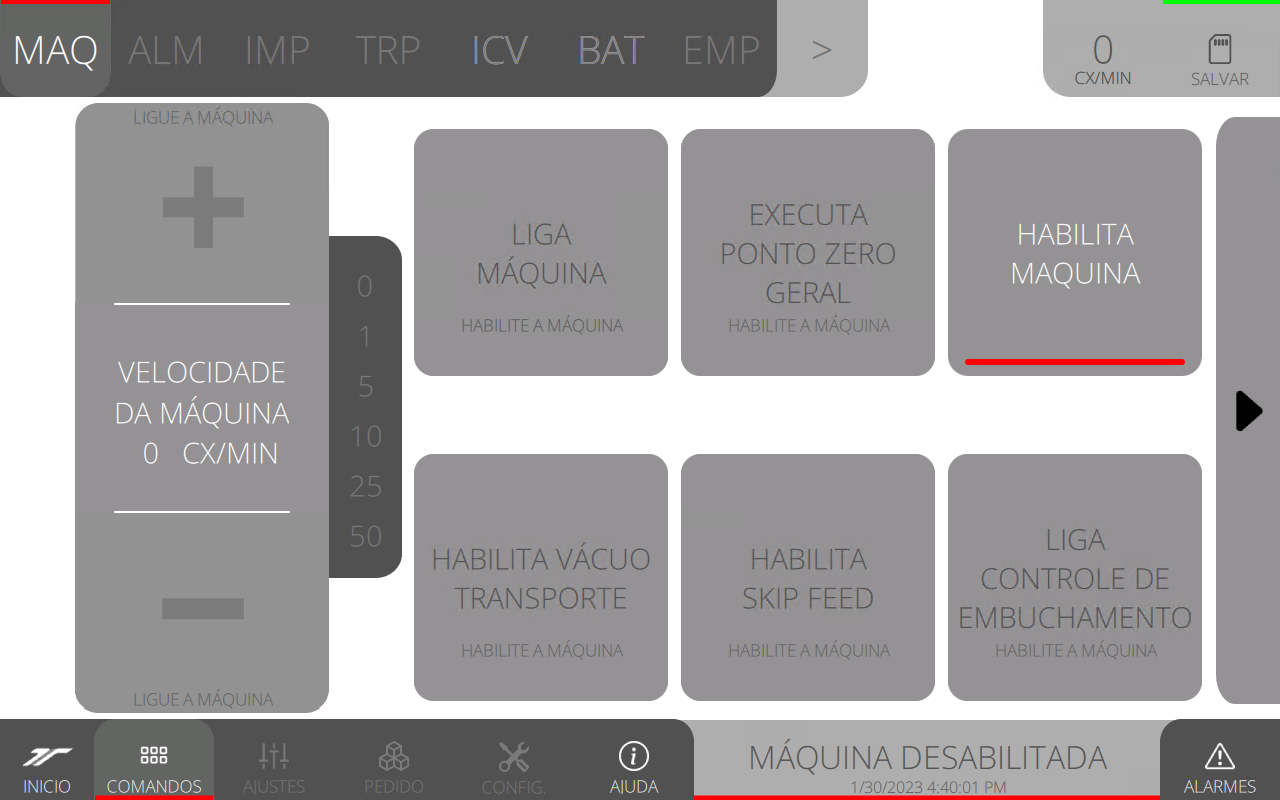
\includegraphics[width=480 px,height=300 px]{src/imagesICV/02-machine/1.png}
\end{figure}
\vspace*{\fill}

\newpage
\thispagestyle{fancy}
\vspace*{40 pt}
\subsubsection{\small{Velocidade da máquina}} \label{sec:comandosMaquinavelocidadeMaquina}
\vspace*{\fill}
\begin{figure}[h]
    \centering
    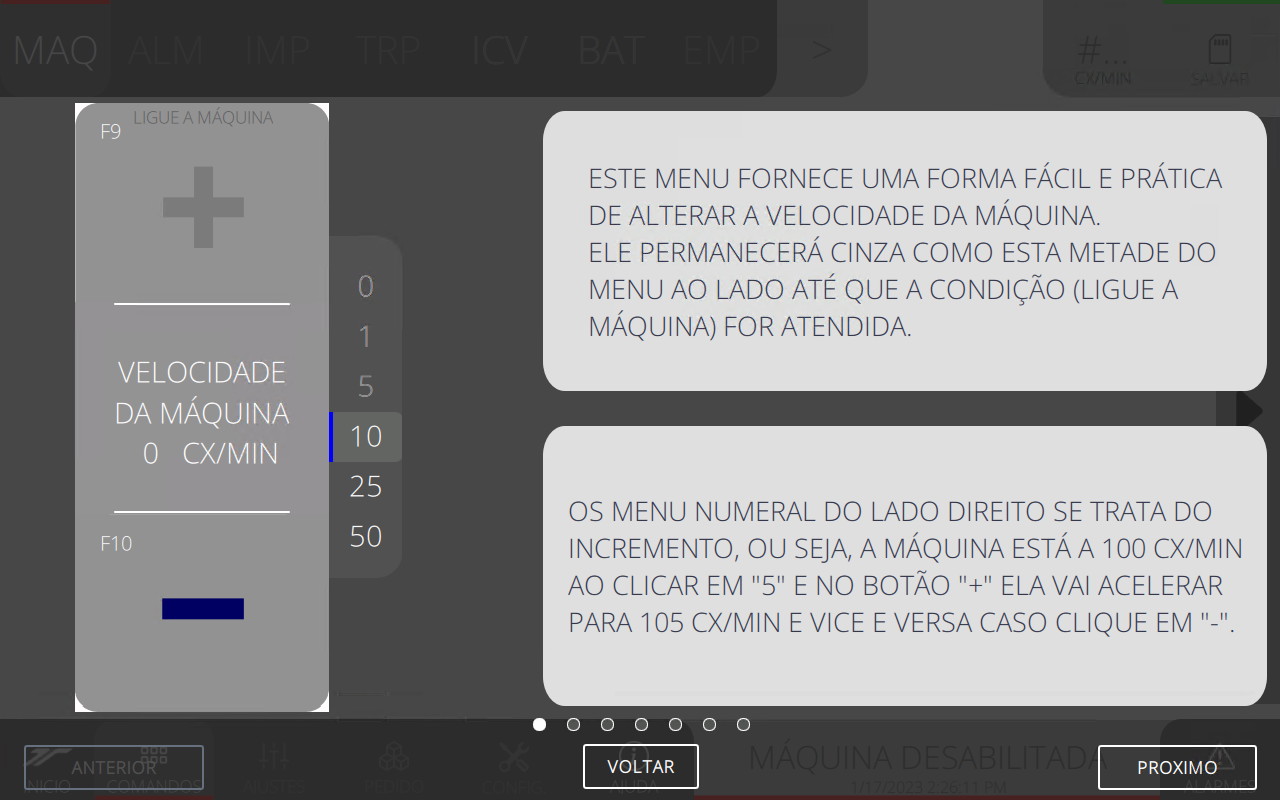
\includegraphics[width=576 px,height=360 px]{src/imagesICV/02-machine/2.png}
\end{figure}
\vspace*{\fill}

\newpage
\thispagestyle{fancy}
\vspace*{40 pt}
\subsubsection{\small{Acionamento da máquina}} \label{sec:comandosMaquinaacionamentoMaquina}
\vspace*{\fill}
\begin{figure}[h]
    \centering
    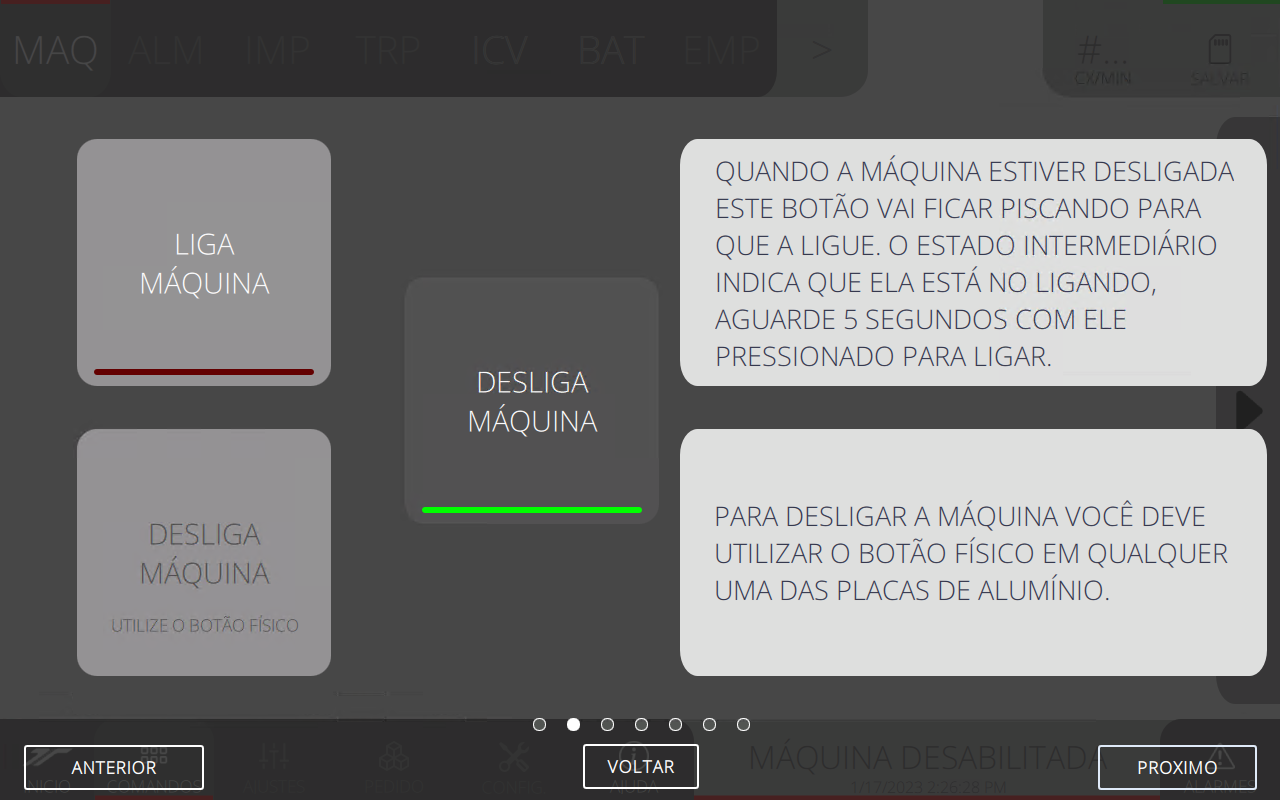
\includegraphics[width=576 px,height=360 px]{src/imagesICV/02-machine/3.png}
\end{figure}
\vspace*{\fill}

\newpage
\thispagestyle{fancy}
\vspace*{40 pt}
\subsubsection{\small{Executa ponto zero geral}} \label{sec:comandosMaquinaexecutaPontoZeroGeral}
\vspace*{\fill}
\begin{figure}[h]
    \centering
    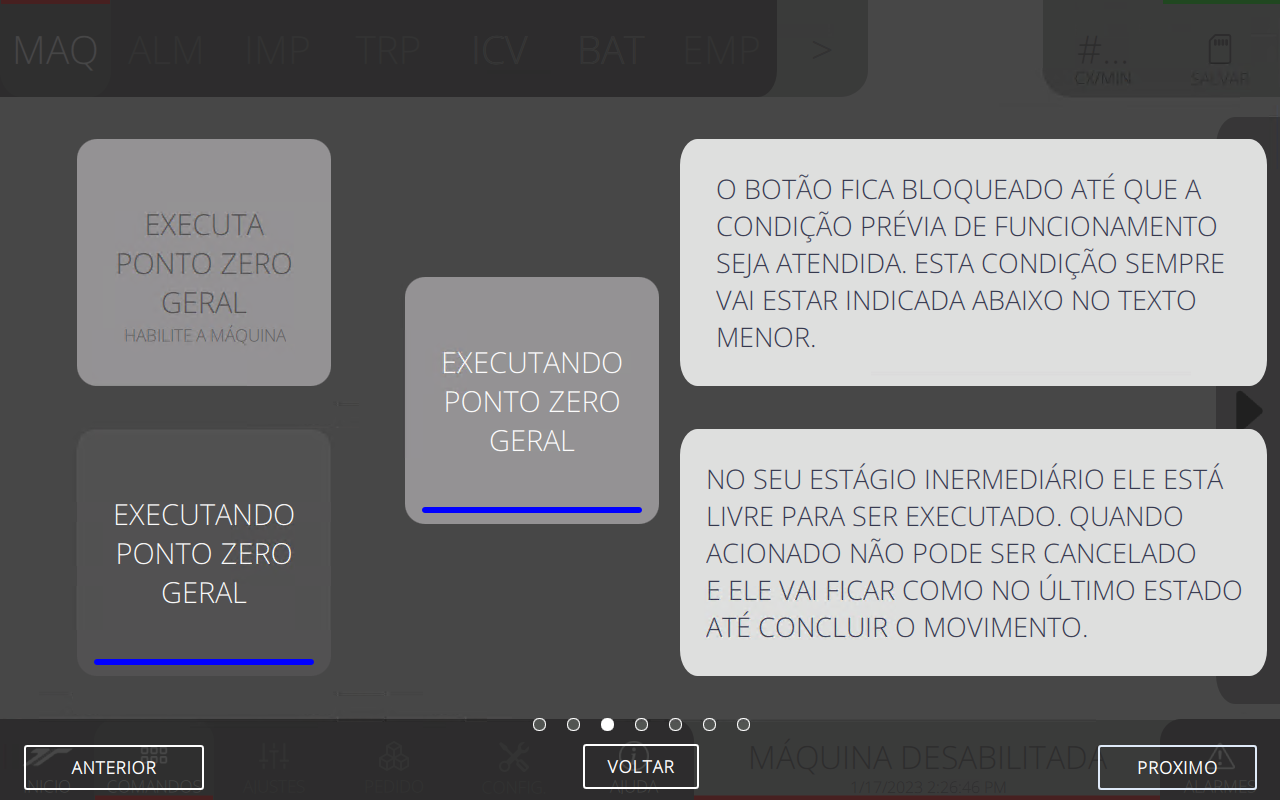
\includegraphics[width=576 px,height=360 px]{src/imagesICV/02-machine/4.png}
\end{figure}
\vspace*{\fill}

\newpage
\thispagestyle{fancy}
\vspace*{40 pt}
\subsubsection{\small{Habilita máquina}} \label{sec:comandosMaquinahabilitaMaquina}
\vspace*{\fill}
\begin{figure}[h]
    \centering
    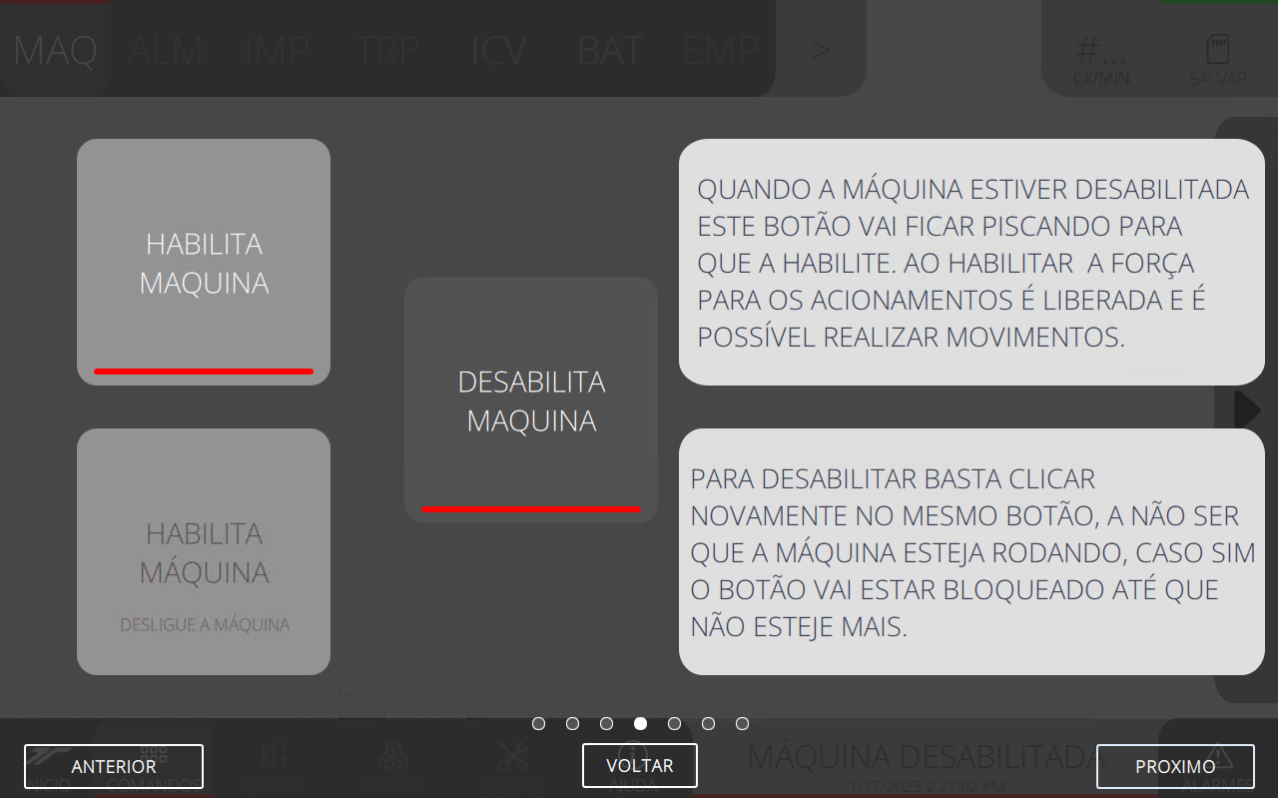
\includegraphics[width=576 px,height=360 px]{src/imagesICV/02-machine/5.png}
\end{figure}
\vspace*{\fill}

\newpage
\thispagestyle{fancy}
\vspace*{40 pt}
\subsubsection{\small{Habilita vácuo transporte}} \label{sec:comandosMaquinahabilitaVacioTransporte}
\vspace*{\fill}
\begin{figure}[h]
    \centering
    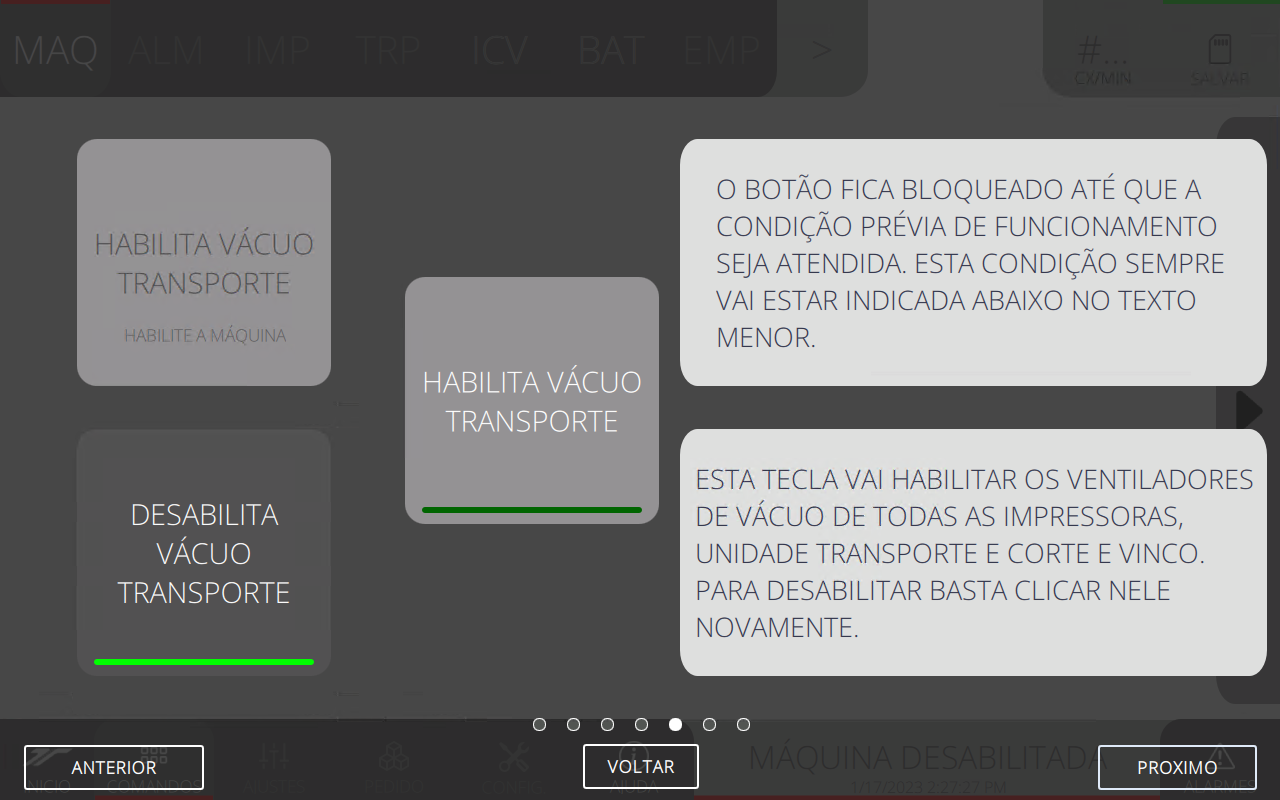
\includegraphics[width=576 px,height=360 px]{src/imagesICV/02-machine/6.png}
\end{figure}
\vspace*{\fill}

\newpage
\thispagestyle{fancy}
\vspace*{40 pt}
\subsubsection{\small{Habilita skip feed}} \label{sec:comandosMaquinahabilitaSkipFeed}
\vspace*{\fill}
\begin{figure}[h]
    \centering
    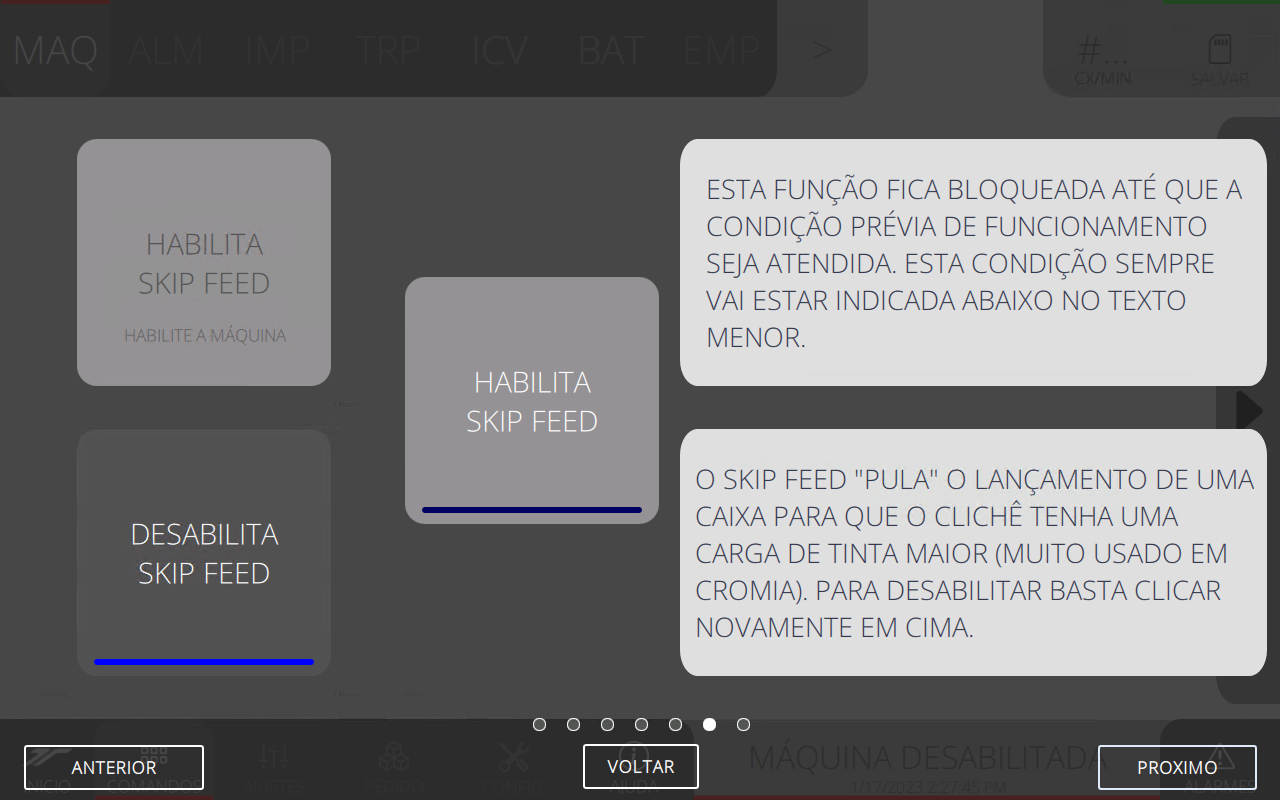
\includegraphics[width=576 px,height=360 px]{src/imagesICV/02-machine/7.png}
\end{figure}
\vspace*{\fill}

\newpage
\thispagestyle{fancy}
\vspace*{40 pt}
\subsubsection{\small{Liga controle do embuchamento}} \label{sec:comandosMaquinaLigaControleDoEmbuchamento}
\vspace*{\fill}
\begin{figure}[h]
    \centering
    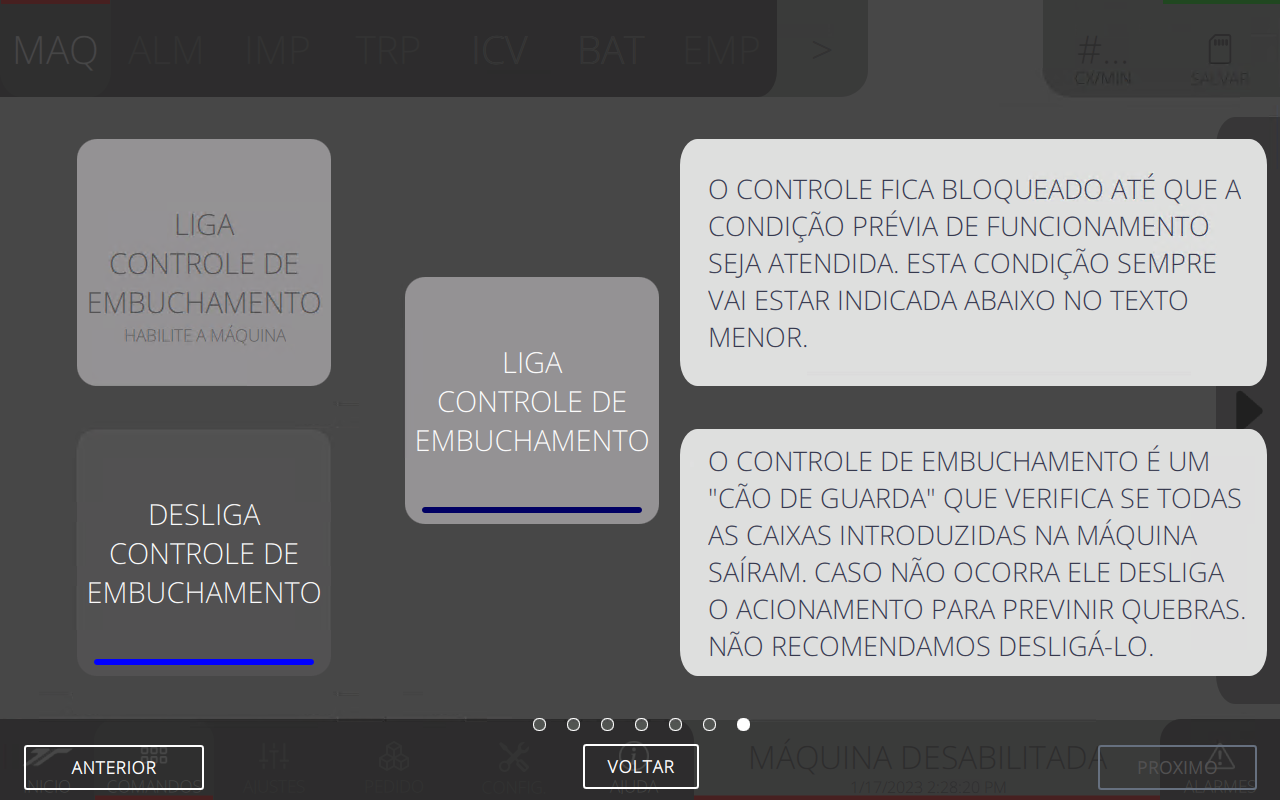
\includegraphics[width=576 px,height=360 px]{src/imagesICV/02-machine/8.png}
\end{figure}
\vspace*{\fill}

\newpage
\thispagestyle{fancy}
\vspace*{40 pt}
\subsection{Segunda tela de comandos da máquina} \label{sec:comandosMaquinaSegundaTela}
Esta tela é acessada clicando no botão "\textgreater" no canto direito da tela de comando da máquina. A lógica de funcionamento dos menus é a mesma da primeira tela de comando da máquina.
\vspace*{\fill}
\begin{figure}[h]
    \centering
    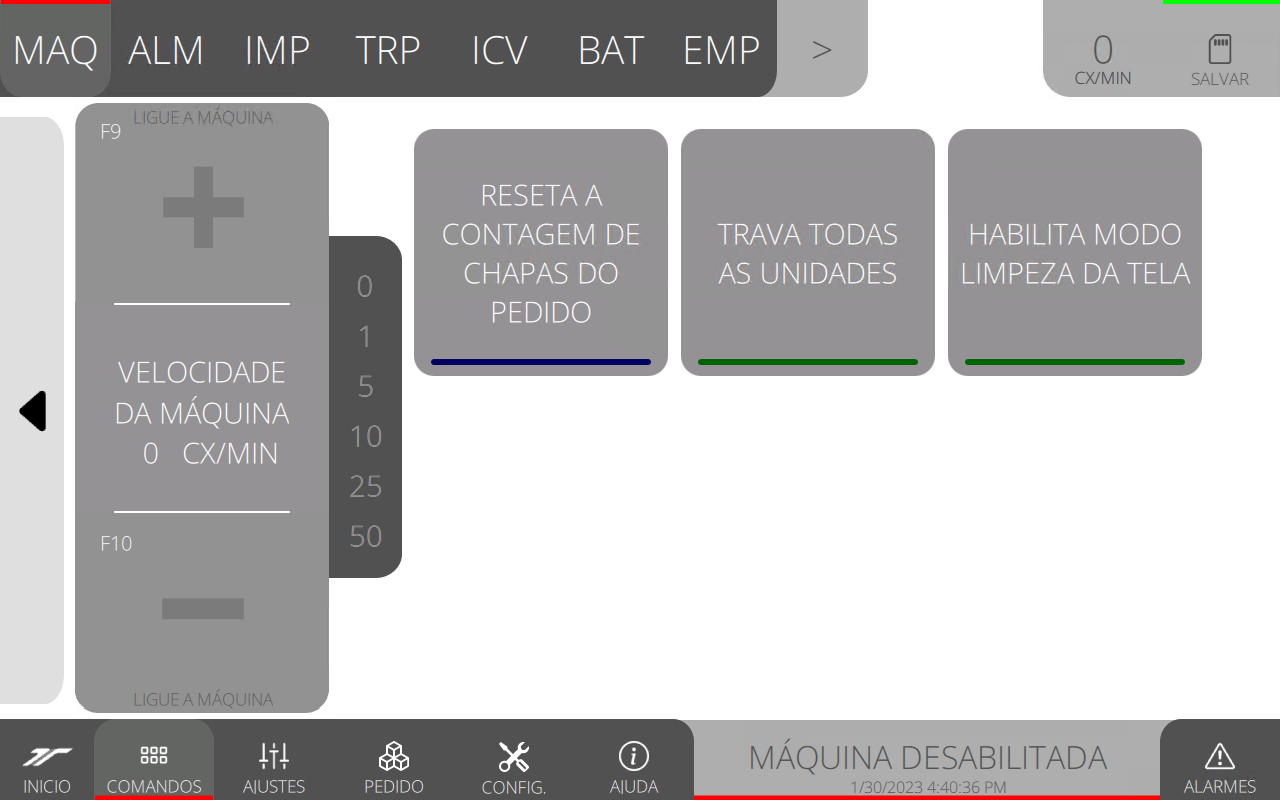
\includegraphics[width=480 px,height=300 px]{src/imagesICV/02-machine/e-Tela-Principal-2.png}
\end{figure}
\vspace*{\fill}

\newpage
\thispagestyle{fancy}
\vspace*{40 pt}
\subsubsection{\small{Trava todas as unidades}} \label{sec:comandosMaquinaTravaTodasAsUnidades}
\vspace*{\fill}
\begin{figure}[h]
    \centering
    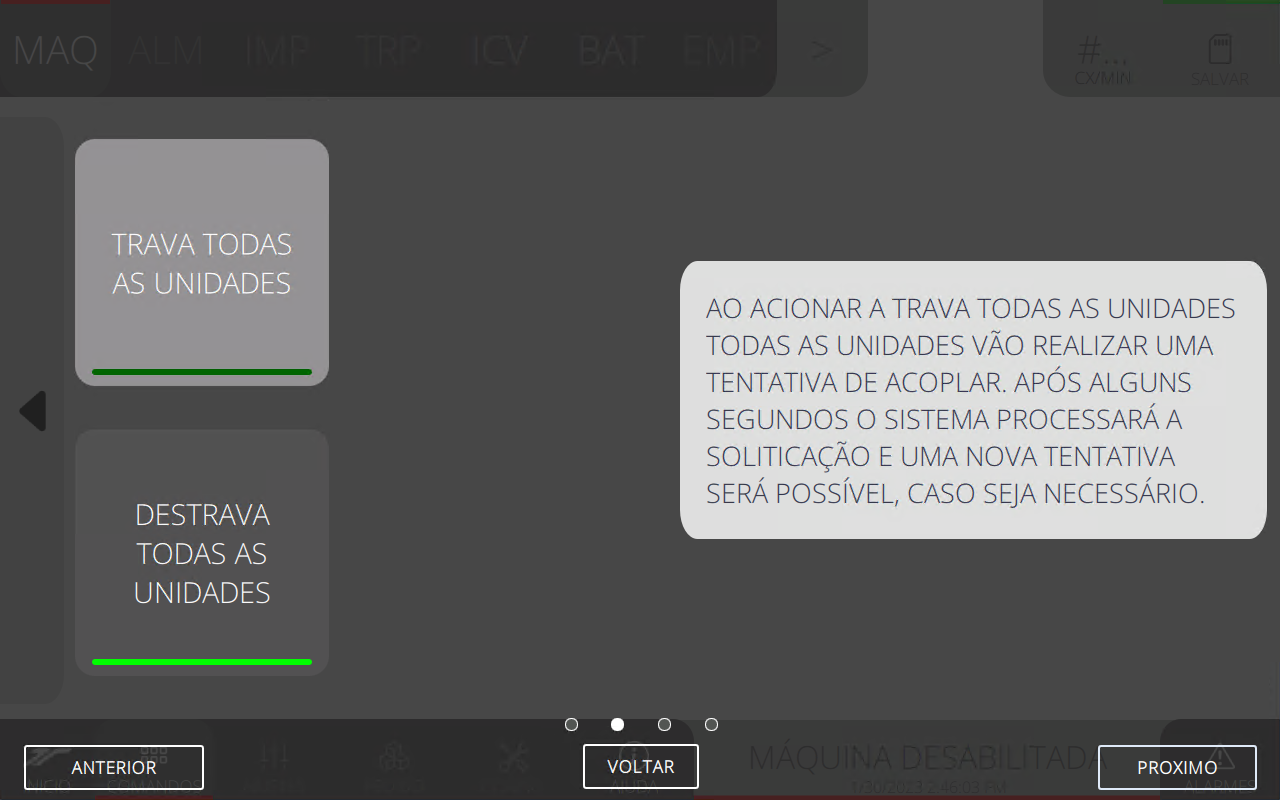
\includegraphics[width=576 px,height=360 px]{src/imagesICV/02-machine/10.png}
\end{figure}
\vspace*{\fill}

\newpage
\thispagestyle{fancy}
\vspace*{40 pt}
\subsubsection{\small{Reseta a quantidade de chapas do pedido}} \label{sec:comandosMaquinaResetaAQuantidadeDeChapasDoPedido}
\vspace*{\fill}
\begin{figure}[h]
    \centering
    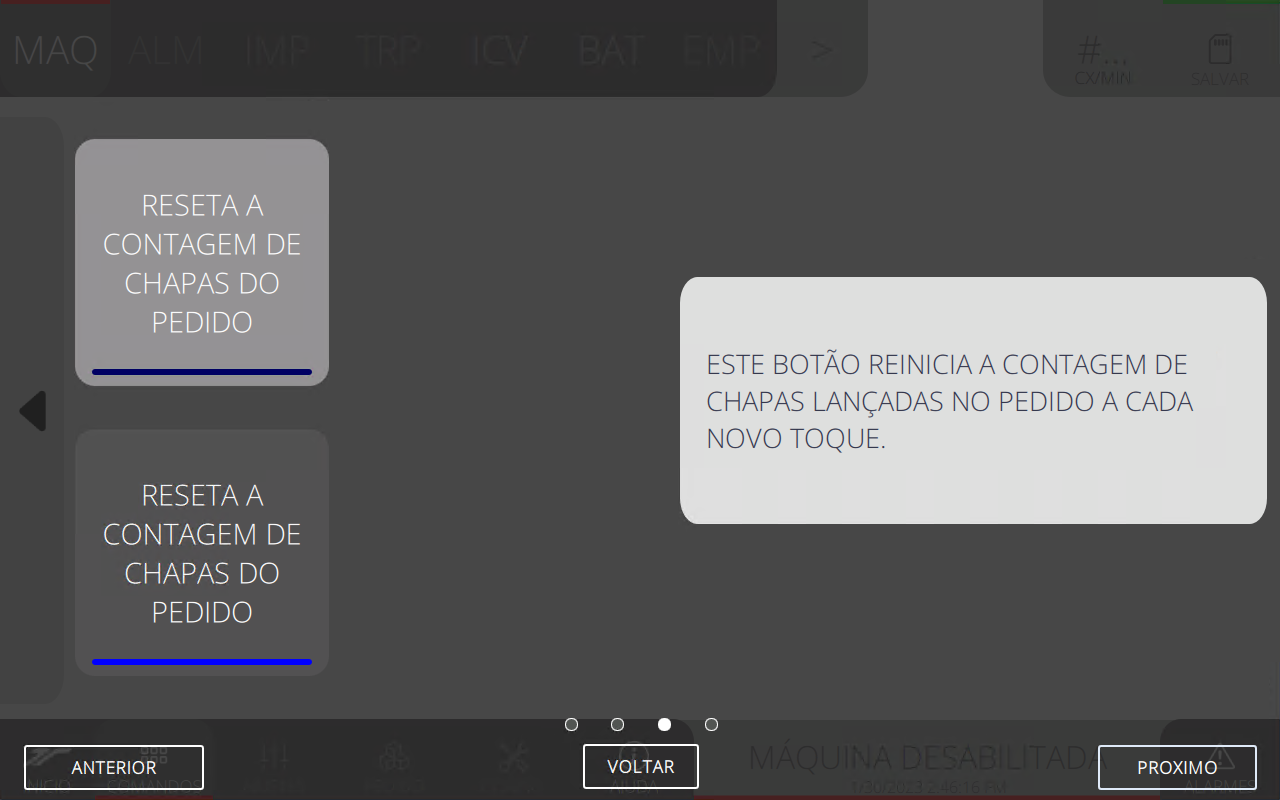
\includegraphics[width=576 px,height=360 px]{src/imagesICV/02-machine/11.png}
\end{figure}
\vspace*{\fill}

\newpage
\thispagestyle{fancy}
\vspace*{40 pt}
\subsubsection{\small{Habilita modo limpeza de tela}} \label{sec:comandosMaquinaHabilitaModoLimpezaDeTela}
\vspace*{\fill}
\begin{figure}[h]
    \centering
    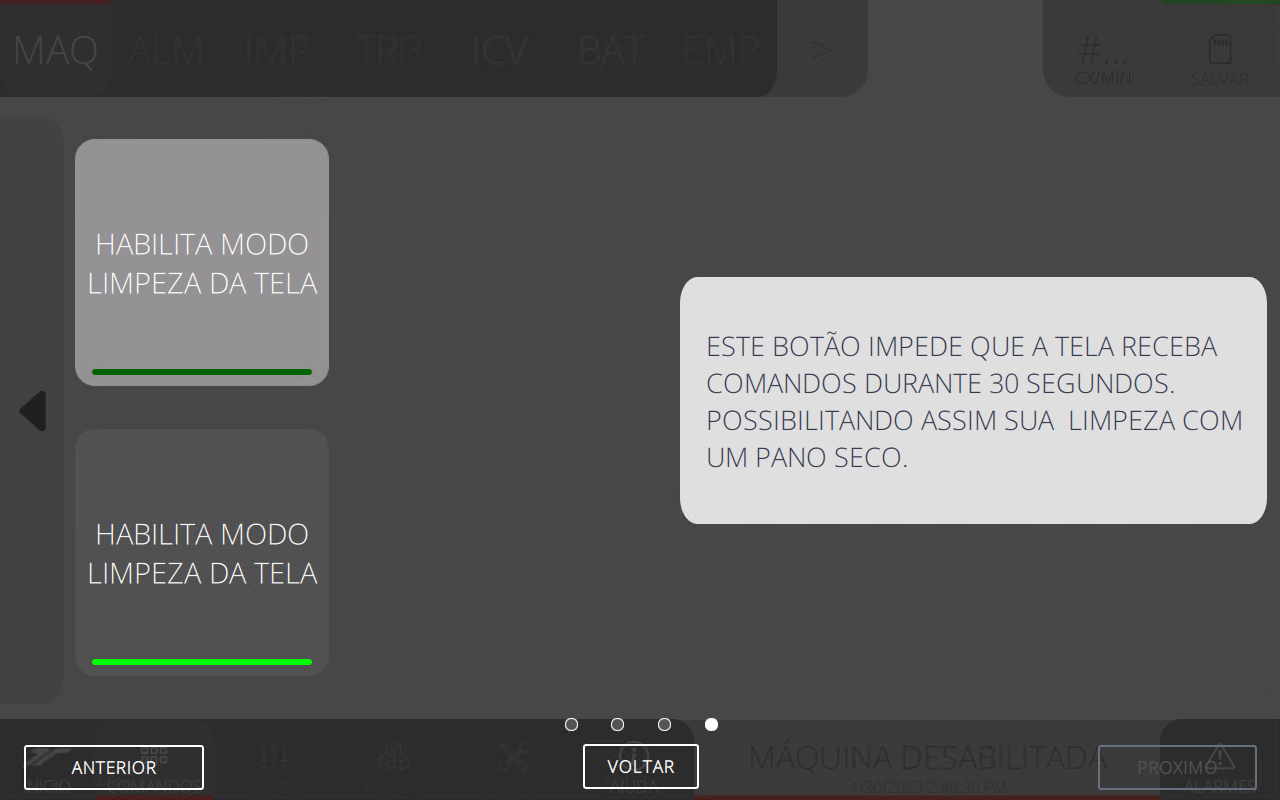
\includegraphics[width=576 px,height=360 px]{src/imagesICV/02-machine/12.png}
\end{figure}
\vspace*{\fill}




